%% Template from Jonas Einarsson, bror.einarsson.net/chalmersthesistemplate/
\documentclass[11pt,a4paper]{report}

% Packages and commands file
\usepackage[utf8]{inputenc}
\usepackage{pdfpages}
%\usepackage[T1]{fontenc}
\usepackage[english]{babel}
%\usepackage{amsmath}
%\usepackage{ae}
%\usepackage{icomma}
%\usepackage{units}
%\usepackage{color}
%\usepackage{graphicx}
%\usepackage{epstopdf}
%\usepackage{subfigure}
%\usepackage{bbm}
\usepackage{caption}
\usepackage{subcaption}
\usepackage{listings}
%\usepackage[square, numbers, sort]{natbib}
%\usepackage{multirow}
\usepackage{array}
%\usepackage{geometry}
\usepackage{fancyhdr}
\usepackage{fncychap}
%\usepackage[hyphens]{url}
\usepackage[breaklinks,pdfpagelabels=false]{hyperref}
%\usepackage{lettrine}
%\usepackage{eso-pic}

\newcommand{\rd}{\ensuremath{\mathrm{d}}}
\newcommand{\id}{\ensuremath{\,\rd}}
\newcommand{\degC}{\ensuremath{\,\unit{^\circ C}}}

% Fancyheader shortcuts
\newcommand{\setdefaulthdr}{
  \fancyhead[L]{\slshape \rightmark}
  \fancyhead[R]{\slshape \leftmark}
  \fancyfoot[C]{\thepage}
}
\newcommand{\setspecialhdr}{
  \fancyhead[L]{ }
  \fancyhead[R]{\slshape \leftmark}
  \fancyfoot[C]{\thepage}
}

\newcommand{\mail}[1]{\href{mailto:#1}{\nolinkurl{#1}}}
\newcommand{\backgroundpic}[3]{
  \put(#1,#2){
    \parbox[b][\paperheight]{\paperwidth}{
      \centering
      \includegraphics[width=\paperwidth,height=\paperheight,keepaspectratio]{#3}
      \vfill
    }
  }
}


% Settings (Metadata)
% References, choose bst-file
\bibliographystyle{elsart-num}

% PDF Metadata and link styles
\hypersetup{
    pdftitle={Master's Thesis: },
    pdfauthor={Alexander Sjösten},
    colorlinks=true,
    citecolor=black,
    filecolor=black,
    linkcolor=black,
    urlcolor=black
}

% preamble for table of contents
\setcounter{tocdepth}{3}
\setcounter{secnumdepth}{3}

% Single page abstract
\renewenvironment{abstract}
{\begin{center} \bfseries \abstractname \end{center}}
{\vspace{2\baselineskip}}


% Single page acknowledgements
\newenvironment{acknowledgements}
{\begin{center} \bfseries Acknowledgements \end{center}}
{\vspace{2\baselineskip}}

% Figure & Table captions
\captionsetup{margin=10pt,font=small,labelfont=bf}
\captionsetup[table]{position=top}
\setlength{\extrarowheight}{4pt}
\addtolength{\headheight}{\baselineskip}

% Fancyheader (see packagescommands.tex for default/special)
\pagestyle{fancy}
\setdefaulthdr

% Stolen settings (unknown origin):
% Alter some LaTeX defaults for better treatment of figures:
% See p.105 of "TeX Unbound" for suggested values.
% See pp. 199-200 of Lamport's "LaTeX" book for details.
%   General parameters, for ALL pages:
\renewcommand{\topfraction}{0.9}	% max fraction of floats at top
\renewcommand{\bottomfraction}{0.8}	% max fraction of floats at bottom
%   Parameters for TEXT pages (not float pages):
\setcounter{topnumber}{2}
\setcounter{bottomnumber}{2}
\setcounter{totalnumber}{4}     % 2 may work better
\setcounter{dbltopnumber}{2}    % for 2-column pages
\renewcommand{\dbltopfraction}{0.9}	% fit big float above 2-col. text
\renewcommand{\textfraction}{0.07}	% allow minimal text w. figs
%   Parameters for FLOAT pages (not text pages):
\renewcommand{\floatpagefraction}{0.7}	% require fuller float pages
% N.B.: floatpagefraction MUST be less than topfraction !!
\renewcommand{\dblfloatpagefraction}{0.7}	% require fuller float pages

% remember to use [htp] or [htpb] for placement


\begin{document}

% Title page, abstract, acknowledgements

\includepdf[pages={-}]{images/frontpage.pdf}
\thispagestyle{empty}

\begin{abstract}
Creating a secure web application with regard to information flow control poses a big challenge and there has been a lot of research in the area of information flow control. When creating a web application, a language like JavaScript is usually used. Since JavaScript is deployed in the browser and can gain access to sensitive information, securing JavaScript application with regards to information flow control is crucial and to help with this, a system called JSFlow has been developed.

However, it is not enough to secure JavaScript with regards to information flow control. Research has been made to help strengthen the weak type system of JavaScript. The research includes creating new languages and creating compilers. The compiler Haste generates JavaScript code from the high-level, strict statically typed language Haskell.

This thesis explores the possibility to create a library in Haskell which enables a static analysis with regards to information flow control. This library should then be compiled with Haste and produce secure JavaScript code with regards to information flow control. In doing so, the compiled code should be able to be run through JSFlow with no halted execution due to information leakage.
\end{abstract}

\newpage
\thispagestyle{empty}

\begin{acknowledgements}
I would like to give thanks to Andrei Sabelfeld for acting as my examiner for this thesis and providing valuable input. I would also like to thank Anton Ekblad for his supervision and sharing his knowledge when giving advice and valuable feedback on the draft of the report; Daniel Hedin for helping out with questions about JSFlow. I would also like to thank my opponents Anders Nordin, Hannes Sandahl and Daniel Eddeland for their feedback during my presentation. Finally, a big thank goes to my all computer scientists in our lunch room Monaden for great laughs and good discussions about everything and nothing. \\[1cm]

\hfill Alexander Sjösten, February 26, 2015, Gothenburg
\end{acknowledgements}


% Table of contents
\newpage
\pagenumbering{roman}
\setcounter{page}{1}
\pagestyle{fancy}
\setspecialhdr
\tableofcontents

% Main area
\newpage
\setdefaulthdr
\pagenumbering{arabic}
\setcounter{page}{1}

% Content
\chapter{Introduction}
\label{chapter:intro}
When developing a web application, there are numerous issues the application writer must consider. One of the most used languages when designing the front-end of a web application is JavaScript~\cite{javascript_popularity}, a dynamically typed, multi-paradigm programming language~\cite{javascript_info}. Unfortunately, JavaScript suffers from a couple of drawbacks and attacks towards the language through Cross-Site Scripting (XSS) were on the third place on the OWASP Top 10 list of most common attacks in 2013~\cite{owasp_xss_rank}. In an XSS attack, the attacker manages to inject JavaScript code into websites that are considered secure~\cite{owasp_xss, excess_xss}. These injections can do anything from harmless pranks (e.g. showing an alert box) to redirecting the non-suspecting user to a fake website to steal valuable information. When an attack like XSS succeeds, the culprit is usually non-escaped input from the users. If a website includes the user input verbatim, an attacker can insert input that will be treated as code by the victim~\cite{excess_xss}. Examples of valuable information retained by the browser for an attacker are cookies and session tokens which can be used to gain access to e.g. personal information and passwords.
\section{Problems with JavaScript}
From a security standpoint with regards to information flow control, JavaScript suffers from two big problems, namely
\begin{itemize}
  \item It uses weak typing, i.e. it does not know at runtime the exact type of a variable or the return type of a function. This is explained more in depth in Chapter~\ref{chapter:weak-dynamic-typing}.
  \item It can gain access to sensitive information from the browser.
\end{itemize}
There are more problems with JavaScript in general, e.g. bad scoping semantics, poor support for the functional paradigm and a lack of modularity. Since those problems are not that important from a information flow security standpoint, it is not in the scope of this report. The curious reader can read more about those problems in~\cite{haste-lang}.

\section{Information Flow Control}
Confidentiality in any system is important. Unfortunately, there are few built in mechanisms for ensuring end-to-end confidentiality policies in programming languages like JavaScript~\cite{ifc-jsac}. The general idea behind information flow control is to tag the data with one of two security levels; \emph{high} or \emph{low}. These levels can be seen as either private data (high security level) or public data (low security level). Figure~\ref{fig:normal_flow} shows the flow in an application developed with the core language of JavaScript. In JavaScript, there is no way of controlling the flow by dividing the different values of the application into either a high or low context. It is more of a straight line from the input to the output. However, if an implementation of a system that enforces information flow control were in place, the flow could be seen as in Figure~\ref{fig:controlled_flow}. The only flow that is not allowed is a flow from a high context to a low context. All the other flows, i.e. low to low, low to high and high to high, are valid. A system that enforces information flow control will help in ensuring end-to-end confidentiality.
\begin{figure}[h]
  \begin{subfigure}{.5\textwidth}
    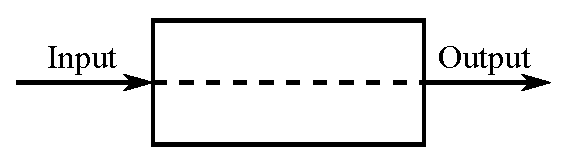
\includegraphics[scale=0.65]{images/flow_normal.eps}
    \caption{Normal information flow}
    \label{fig:normal_flow}
  \end{subfigure}
  \begin{subfigure}{.5\textwidth}
    
\includegraphics[scale=0.65]{images/flow_controlled.eps}
    \caption{Controlled information flow}
    \label{fig:controlled_flow}
  \end{subfigure}
  \caption{Different kinds of flow in a web application}
  \label{fig:flows}
\end{figure}

\newpage
\clearpage
\chapter{Background}
As mentioned in Chapter~\ref{chapter:intro}, JavaScript has several shortcomings. This chapter will explain those shortcomings in more detail. It will also introduce two of the tools that will be used in this project; Haste~\cite{haste-lang} and JSFlow~\cite{jsflow,jsflow-csf12,jsflow-sac14}. Finally, some terminology and related work will be presented.

\section{Problems with JavaScript - part deux}
As mentioned in Chapter~\ref{chapter:intro}, from a security standpoint JavaScript suffers from weak dynamic typing and having access to sensitive information in the browser.
\subsection{Weak dynamic typing}
\label{chapter:weak-dynamic-typing}
There are several odd features one can use in JavaScript due to the weak dynamic typing. Where a statically typed language (e.g. Java) would give a compile error, the JavaScript code will be run and perhaps succeed but with unexpected results. Figure~\ref{fig:error_java} shows a logical error that is caught at compile time in Java. If the code in Figure~\ref{fig:error_java} would be allowed to run, it would be up to the runtime environment to determine how the code would be interpreted. The same error in JavaScript is shown in Figure~\ref{fig:error_js}. Since JavaScript does not have any static type checking the decision on how to interpret the code will be made at runtime. Instead of failing and raising a runtime error, JavaScript will convert the \textbf{true} value into a number which in this case corresponds to the number \textbf{1}. Hence the addition will be evaluated to \textbf{3}. Situatuations like that, where a clear type error is allowed to propagate and potentially change the state of the application should be considered dangerous and prone to producing bugs.

Another issue with the weak type system in JavaScript can be seen in Figure~\ref{fig:js_comparison}. It is perfectly legal to compare a function with an array in JavaScript. The code in Figure~\ref{fig:js_comparison} will evaluate to \textbf{true}. This can in turn make it very difficult to find potential bugs since JavaScript will try to convert values of different types to the same types and then make the comparison. In e.g. Java, the comparison in Figure~\ref{fig:js_comparison} would not go through the type checker.
\begin{figure}[h]
  \begin{verbatim}
    int a = 2;
    boolean b = true;
    a + b;  // This should not be allowed to be run
  \end{verbatim}
  \caption{Logical error in Java}
  \label{fig:error_java}
\end{figure}
\begin{figure}[h]
  \begin{verbatim}
    var a = 2;
    var b = true;
    a + b;  // This will evaluate to 3
  \end{verbatim}
  \caption{Logical error in JavaScript}
  \label{fig:error_js}
\end{figure}
\begin{figure}[h]
  \begin{verbatim}
    (function(x) { return x * x; }) > [1,2,3];
  \end{verbatim}
  \caption{Weird comparison in JavaScript}
  \label{fig:js_comparison}
\end{figure}

\subsubsection{Attempts to solving the type problem}
There have been several attempts of providing a more secure type system to JavaScript, everything from creating a statically typed language that compiles to JavaScript to a compiler from an already existing programming language and compile it to JavaScript to a static type checker. Examples of attempted soultions are
\begin{itemize}
  \item \textbf{TypeScript}~\cite{typescript}, a typed superset of JavaScript that compiles to plain JavaScript.
  \item \textbf{TeJaS}~\cite{tejas-art,tejas-git}, which allows you to annotate type signatures as comments in the JavaScript code and then type checks the code.
  \item \textbf{GHCJS}~\cite{ghcjs} and \textbf{Haste}~\cite{haste-lang,haste-symposium}, which compiles from Haskell, a statically typed, high-level functional programming language~\cite{haskell}, to JavaScript.
\end{itemize}

\subsection{Sensitive information in the browser}
The browser has access to several different types of sensitive information and can be used by an attacker to get the sensitive information. JavaScript can gain access to e.g. cookies, send HTTP requests and make arbitrary DOM modifications. If untrusted JavaScript is executed in a victim's browser, the attacker can, among other things, perform the following attacks:
\begin{itemize}
  \item \textbf{Cookie theft}, where the attacker can gain access to the victim's cookies that are associated with the current website.
  \item \textbf{Keylogging}, where the attacker can create and register a keyboard event listener and send the keystrokes to the attacker's own server in order to potentially record passwords, credit card information etc.
  \item \textbf{Phishing}, where the attacker can insert fake forms by manipulating the DOM and fool the user to submit sensitive information which will be redirected to the attacker.
\end{itemize}
\subsubsection{Attempts to solving the information problem}
The current solution to secure the sensitive information JavaScript has access to as of now is to sandbox the script and run it in a secure environment. There are mainly three ways of doing this.
\begin{itemize}
  \item Wrap the script inside a call to with and pass a faked window object and execute the code with eval.
  \item Use an iframe and set the sandbox attribute to either not allow scripts to run or have it be run within that iframe only. Unfortunately, as explained in~\cite{js_in_js}, iframes have some issues as well.
  \item Use existing tools to help sandbox third party code, such as:
    \begin{itemize}
      \item \textbf{JavaScript in JavaScript}~\cite{js_in_js}, an interpreter that allows an application to execute third-party scripts in a completely isolated, sandboxed environment.
      \item \textbf{Caja}~\cite{caja_spec}, a compiler to make third party code safe to embed within a website.
    \end{itemize}
\end{itemize}
\section{Haste}
Haste (HASkell To Ecmascript compiler) is a compiler that compiles the high-level language Haskell to JavaScript. The Haste compiler is plugged into the compilation process from GHC, the Glasgow Haskell Compiler. As can be seen in Figure~\ref{fig:system}, Haste starts its compilation process after GHC has done some code optimization. From the optimized code from GHC, Haste will create an AST, Abstract Syntax Tree, for JavaScript. The AST will then be optimized and after the optimization process in Haste is done the actual JavaScript code will be generated.
\begin{figure}[h]
  \begin{tabular}{|c|c|c|}
    \hline
    Step & Operation & GHC/Haste \\
    \hline
    1 & Parse & GHC \\
    2 & Type check & GHC \\
    3 & Desugar & GHC \\
    4 & Intermediate code generation & GHC \\
    5 & Optimization & GHC \\
    6 & Intermediate code generation (JS AST) & Haste \\
    7 & Optimization & Haste \\
    8 & Code generation to JavaScript & Haste \\
    \hline
  \end{tabular}
  \caption{The compilation process for the Haste compiler}
  \label{fig:system}
\end{figure}

When compiling the Haskell source code with Haste, the compilation process will result in a JavaScript file. If Haste.App is used, the compilation process will create the source code for the client in JavaScript and a server binary~\cite{haste-symposium}.

\section{JSFlow}
JSFlow is an interpreter written in JavaScript that dynamically checks the JavaScript code at runtime to ensure information flow security. Currently, JSFlow supports full information flow control for ECMA-262 v5 apart from strict mode and JSON.

Within information flow security, there are two types of flow that must be checked - explicit flow and implicit flow. Even though there are several different ways an attacker can gain information about a system (e.g. via timing attacks), only explicit and implicit flows for computations are considered. JSFlow does not provide security for e.g. timing attacks and due to this, handling timing attacks will be outside of the scope for this thesis.
\subsection{Explicit flow}
With explicit flow, one means when a data in a \emph{high} context leaks information to a \emph{low} context explicitly. An example can be seen in Figure~\ref{fig:expflow} where the value of the high variable \emph{h} is leaked to the low variable \emph{l}. Obviously this should be illegal when information flow security is applied and explicit flows are not difficult to find when dynamically checking the code. When data is written to a variable, one simply must keep track of the context of the variable and the context of the data. If the variable is in low context and the data is in high context an error should be produced and execution of the JavaScript code should be stopped. All other scenarios (high variable with high data, high variable with low data and low variable with low data) are allowed.
\subsection{Implicit flow}
\label{chapter:implicit_flow}
Implicit flows occurs when e.g. a language's control structure is used in combination with side effects to leak information. Figure~\ref{fig:impflow} shows an example of an implicit flow. The variable \emph{l} will get the value 1 if and only if the variable \emph{h} is an odd number. Otherwise \emph{l} will have the value 0. A dynamic system that will handle implicit flows must associate a security context with the control flow~\cite{jsflow-csf12}. In Figure~\ref{fig:impflow}, the body of the if statement should be executed in a secure context and therefore the variable \emph{l} must be a secure variable in order for the flow to be valid.

\begin{figure}[h]
  \captionsetup[subfigure]{singlelinecheck=off,justification=raggedright}
  \begin{subfigure}[b]{0.5\textwidth}
    \begin{verbatim}
      l := h
    \end{verbatim}
    \caption{Explicit flow}
    \label{fig:expflow}
  \end{subfigure}
  \begin{subfigure}[b]{0.5\textwidth}
    \begin{verbatim}
      h := h mod 2;
      l := 0;
      if h = 1 then l := 1;
      else skip;
    \end{verbatim}
    \caption{Implicit flow}
    \label{fig:impflow}
  \end{subfigure}
  \caption{Implicit and explicit flow}
\end{figure}

\subsection{Example of coding for JSFlow}
When creating a web application in JavaScript that JSFlow should be able to check, there is only one function that the programmer must know about - the \emph{upg} function. The function upg is used when lifting a computation into a high context. In Figure~\ref{fig:upg}, the variable \emph{h} is lifted into a high context by calling upg on the data to be stored to \emph{h}. Due to the call to upg, the variable h will be a high variable containing the number 42. As can be seen with the variables \emph{l}, which is a low variable, and \emph{t}, which is a high variable, the default level for a compuation is low unless JSFlow infers that a variable \textbf{must} be high due to part of the compuation being high.

\begin{figure}[h]
  \begin{verbatim}
    // Variable l is a low variable of value 2
    var l = 2;

    // Variable h is a high variable of value 42
    var h = upg(42);

    /* Variable t must be a high variable due to h
       being high */
    var t = l + h;
  \end{verbatim}
  \caption{Creating high and low variables in JavaScript with JSFlow}
  \label{fig:upg}
\end{figure}
The {\tt upg} function will take a computation (in Figure~\ref{fig:upg} the compuation is simply the number 42) and bind that value to the assigned variable (in Figure~\ref{fig:upg} the variable {\tt h}) and put the variable in a high context.

\subsection{Flows in a pure functional language}
Even though there are two different flows in JavaScript (implicit and explicit flows), there is only one type of flow in a pure functional programming language like Haskell, an explicit flow~\cite{seclib}. As described in Chapter~\ref{chapter:implicit_flow}, an implicit flow depends on control structures in combination with side effects in order to leak information. However, even though a pure functional programming language like Haskell contains control structures, a pure function does not contain side effects. A control structure like an if-statement can be interpreted as a regular function returning a constant value. This means that a function like
\begin{verbatim}
    f :: HInt -> LInt
    f x = if x `mod` 2 == 0
              then 42
            else -42
\end{verbatim}
will look like an implicit flow but is in fact an explicit flow. Note that, in this case {\tt HInt} stands for a \emph{High Int} and {\tt LInt} stands for a \emph{Low Int}. An if-then-else can be rewritten as a regular function~\cite{if-then-else}
\begin{verbatim}
    myIf :: Bool -> a -> a -> a
    myIf True  b1 _ = b1
    myIf False _ b2 = b2
\end{verbatim}
where {\tt b1} and {\tt b2} are the different branches. The different branches are of type {\tt a}, which in this case can be any arbitrary expression. Rewriting the function {\tt f} using {\tt myIf} can be done as follows:
\begin{verbatim}
    f :: HInt -> LInt
    f x = myIf (x `mod` 2 == 0) 42 (-42)
\end{verbatim}
where a constant value, either {\tt 42} or {\tt -42}, is returned. Since there are no side effects in a pure function like {\tt f}, there can be no implicit flows. Every flow will be explicit, which in turn makes it easier to create a structure in the type system that keeps track of the flow.

\section{Non-interference}
The principles of non-interference were introduced by Goguen and Meseguer in 1982~\cite{non-interference-goguen-meseguer} who defined non-interference to be
\newline
\begin{center}
  \emph{one group of users, using a certain\\set of commands, is noninterfering\\with another group of users if what\\the first group does with those\\commands has no effect on what the\\second group of users can see.}
\end{center}
When talking about non-interference with regards to information flow control, one means a property that states that the public outcome does not depend on any private input. An attacker should not be able to distinguish between two computations from their outputs if the computations only vary in the secret input.

As an example of non-interference, assume the following function where something of type \textbf{Char} is of high value and something of type \textbf{Int} is of low value:
\begin{verbatim}
    fOk :: (Char, Int) -> (Char, Int)
    fOk (c, i) = (chr (ord c + i), i + 42)
\end{verbatim}
The function {\tt fOk} preserves confidentiality since it does not leak any valuable information about the value {\tt c}. In this case, preserving the confidentiality of {\tt c} means that no information of {\tt c} is leaked. It is said to be \emph{non-interfered} since the public result (the Int value) is independent of the value of {\tt c}. If the function instead was defined as
\begin{verbatim}
    fBad1 :: (Char, Int) -> (Char, Int)
    fBad1 (c, i) = (c, ord c)
\end{verbatim}
it would not be non-interfered because the confidentiality is broken. Information about {\tt c} is leaked through the low Int and the corresponding decimal value of the ASCII number of {\tt c} is returned as the second value of the tuple.

Unfortunately, information leakage is seldom as explicit as in the {\tt fBad1} function. An attacker might be clever and attempt
\begin{verbatim}
    fBad2 :: (Char, Int) -> (Char, Int)
    fBad2 (c, i) = (c, if ord c > 31 then 1 else 0)
\end{verbatim}
which would give information about whether or not the variable {\tt c} is a printable character (the ASCII values of printable characters start at 32~\cite{ascii})~\cite{seclib}. Just as with {\tt fBad1}, {\tt fBad2} does not satisfy the non-interference property.

\section{Declassification}
\label{chapter:declassification}
A system that satisfies the non-interference policy is a very strict system. A system usually needs some kind of controlled release of confidential data. As an example, imagine a login system. A user's password should be handled as confidential data when the user attempts to login. If the login succeeded the user should be authenticated and redirected whereas if the login failed the user should be prompted with a message saying the username/password combination was incorrect. If the system was non-interfered, there could be no message explaining to the user that the username/password was incorrect since that output would rely on confidential data. Another example could be when a credit card is being used for online payment. In the order receipt it is not uncommon to include the last four digits of the credit card number. Again, this is something that can not be done if the system is non-interfered since a credit card number should be considered confidential.

Unfortunately, there is no way for the non-interference policy to distinguish between intended release of information and release that occurs due to an attack or programming error. In order to allow controlled information leak one can use declassification policies.
Taking the example of the credit card explained above and assuming a function \emph{getLastFour} that takes a secret credit card number \emph{h} as an argument and returns a secret value containing the last four digits of the credit card number, producing an intended information release to the variable \emph{l} can be achieved by calling a \emph{declassify} function:
\begin{verbatim}
    l := declassify(getLastFour(h))
\end{verbatim}
However, just allowing declassification everywhere can be dangerous. In theory, an attacker could compromise the declassification and extract more information than intended. Due to this, work on classifying the declassification into four different dimensions has been presented in~\cite{declassification-dimensions}. The proposed dimensions are
\begin{itemize}
  \item \textbf{What} information is released.
  \item \textbf{Who} controls the information release.
  \item \textbf{Where} in the system the information is released from.
  \item \textbf{When} the information is released.
\end{itemize}
and these should be seen as recommendations for how to build the declassification policies in systems.
\section{Related Work}
\label{chapter:related}
There has been research within information flow control and libraries have been created in order to help enforce information flow policies and secure both confidentiality and integrity of the information. Some of the most relevant findings for this project will be described below.
\subsection{LIO}
LIO (Labeled IO) is a library created in Haskell for dynamic information flow control~\cite{lio-2011}. Compared to the library created for this thesis, LIO keeps track of a \emph{current label}, which is an upper bound of the labels of all data that can be observed or modified in the evaluation context. One can also bound the current label with a \emph{current clearance}, where the clearance of a region of code can be set in advance to provide an upper bound of the current label within that region. LIO attempts to close the gap with static analysis, which even though it has its advantages (fewer run-time failures, reduced run-time overhead etc.) has a problem when new kinds of data (e.g. user input) can be encountered at runtime, and dynamic systems.
\subsection{Seclib}
Seclib is a light-weight library for information flow control in Haskell~\cite{seclib, seclib_git}. Just as with the library created in this thesis, Seclib is based on monads and all private data lives within the created monad. However, compared to the library in this thesis, Seclib creates two different monads, \textbf{Sec} and \textbf{SecIO}, where SecIO is an extended IO monad (an IO monad wrapped in a Sec monad). Seclib was designed to be a small, lightweight library and consists, as of Jan. 29 2015, of only 342 lines of code.
\subsection{LMonad}
LMonad~\cite{lmonad} is a library tailored to provide information flow control for web applications written in Yesod, a framework for creating web applications in Haskell~\cite{yesod}. It is a generalization of LIO and provides a Monad Transformer~\cite{monad-transformer}, which in theory means it can be "wrapped around" any monad. Programmers can define their own information flow control policies and after defining them, LMonad guarantees that database interacions follow the policies.
\subsection{RDR}
RDR is a monad which builds on the DLM (Decentralized Label Model) to provide information flow control. DLM allows declassification in a decentralized way~\cite{dlm} and consists of four important parts~\cite{dlm-site}:
\begin{itemize}
  \item \emph{Principles}, which is an entity with power to change and observe certain aspects of the system. A principle \emph{p} can delegate authority to a principle \emph{q} and the actions taken by \emph{q} is implicitly assumed to be authorized by \emph{p}. The principals can have different security policies which makes the system modular.
  \item \emph{Reader policy}, which allows the owner of the policy to specify which principals who are allowed to read a given piece of information. This is a \emph{confidentiality policy}.
  \item \emph{Writer policy}, which allows the owner of the policy to specify which principals who may have influenced the value of a given piece of information. This is an \emph{integrity policy}.
  \item \emph{Labels}, which is a pair of a confidentiality policy and an integrity policy. It is the labels that are used to anotate programs.
\end{itemize}

The purpose of RDR is to extend restricted delegation and revocation to information flow control. The main principle is to allow information flow to a predefined chain of principals, but keeping a right to revoke it at any time. The RDR monad is built by using a Reader monad over the IO monad. One of the ideas of RDR is to see restricted delegation as declassification and protected values should only be allowed to be read by using a valid principal and due to the DLM, mutually-distrusting principals should be allowed to express individual confidentiality and integrity policies~\cite{rdr}.
\subsection{Why another library?}
As explained above, there are already working libraries for information flow control so why would another library be needed? Even though the current libraries are good, they lack one part - integration with a dynamic system. The library will help close the gap between static control for information flow control and already created tools for dynamic check of information flow control (JSFlow) and created tools for securing JavaScript from the viewpoint of a type system (Haste).

% The created library will be able to be run in GHC if one wants to create a system strictly for Haskell but it should also be able to run the code with Haste and as a result get produced JavaScript code which is tagged so JSFlow can dynamically track the information flow.  <-- För abstract..? Eller kanske introduction?

\newpage
\clearpage
\chapter{Goal and limitations}
This chapter will describe the goals and limitations of the thesis.

\section{Goal}
The goal of the thesis is to create a library that will help close the gap between static and dynamic checks for information flow control. In particular, this will be done by extending Haste to produce JavaScript code targeting JSFlow.

\section{Limitations}
The following areas will not be considered in this thesis:
\begin{itemize}
  \item DOM support.
  \item Support for Haste.App, which will include HTML5 with Websockets.
  \item Dynamic information flow control.
  \item Side-channel attacks towards a system (e.g. timing attack).
  \item Securing any communication outside of the JavaScript that is to be generated by Haste.
  \item More than two security levels.
\end{itemize}

\newpage
\clearpage
\chapter{Prototypes}
\label{chapter:prototypes}
For this project, three different prototypes were developed. There are not many differences between the non-monadic and the monadic version and for the final implementation the monadic version was chosen.
\section{Embedded Domain Specific Language}
The first prototype developed was a deeply embedded domain specific language (\emph{EDSL})~\cite{haskell_edsl}. In theory, an EDSL is a embedded language within another language. In this case, the library would be a EDSL within Haskell. In a deep EDSL, an abstract syntax tree is created to represent a program while in a shallow EDSL, language constructs are mapped directly to their semantics~\cite{haskell-deep-shallow}.

In the prototype, the different operations allowed were translated to constructors of a data type called {\tt Expr}, where {\tt Expr} represented expressions. Even though an EDSL is very powerful it suffers from a major drawback. It is difficult to gain access to features from the main language. An example is recursion, something that exists in Haskell, that needs to be implemented again within the EDSL (usually as a constructor which needs to be interpreted). Due to the constraint of not being able to use language-specific features without implementing them again and the increased overhead of defining every action that should be allowed within a datatype, this prototype was quickly disposed of.

\section{Non-monadic}
In the non-monadic prototype, the first thing that needed to be tested was different implementations for a type that defines a flow. The first version can be seen in Figure~\ref{fig:first_flow} and contained a \emph{State monad} from a tuple containing a \emph{tag} and a value to an \emph{internal state}. The internal state were to keep track of the program counter ({\tt pc}) and all active scopes ({\tt activeScopes}). By keeping track of an internal state and the program counter, one could check if a computation leaks information or not. This has several drawbacks. First, it is complex; a program counter and keeping track of the internal state are not needed for a statical analysis - it can be done within the type system of Haskell. Second, keeping track of every variable is very tedious from the library that is to be created since Haste will generate variable names when the application is compiled. Having a dynamic representation of variable names within the created library will therefore not be necessary.
\begin{figure}[h]
  \begin{verbatim}
    type Ident = String
    type Scope a = Map Ident (Tag, Term a)

    data Tag = High | Low
    
    data InternalState a = InState { pc :: Tag
                                   , activeScopes :: [Scope a]
                                   }

    newtype Flow level a = Flow (State (level, a) (InternalState a))

    data LType a where
      LInt    :: Tag -> Int    -> LType (Tag, Int)
      LString :: Tag -> String -> LType (Tag, String)
      LBool   :: Tag -> Bool   -> LType (Tag, Bool)

    data Term a where
      TType :: Term (LType a)
      TApp  :: Term a -> Term a

  \end{verbatim}
  \caption{First attempt at a Flow type}
  \label{fig:first_flow}
\end{figure}

The prototype shown in Figure~\ref{fig:first_flow} was revised to what is shown in Figure~\ref{fig:second_flow}. As in Figure~\ref{fig:first_flow}, it contained a State monad but this time it was from a tuple containing a tag and a value to a list of tuples of tags and values. In principle, a state is used to keep track of the different data values (i.e. computations) and their respective tags. This would then be used to ensure that no information was leaked. Since Haste makes a lot of computations that is encapsulated within the IO monad, it was later decided to have the Flow type use the IO monad instead of the State monad. How Flow was implemented can be seen in Chapter~\ref{sec:flow}.
\begin{figure}[h]
  \begin{verbatim}
    newtype Flow tag a = Flow (State (tag, a) [(tag, a)])
  \end{verbatim}
  \caption{Second attempt at a Flow type}
  \label{fig:second_flow}
\end{figure}

In order to use the Flow type properly, several help functions were implemented. It turned out that one of the help functions was similar to the \emph{bind operator} for monads while other help functions were similar to the functions in the \emph{Applicative} and \emph{Functor} instances. With that in mind, the logical step was to attempt to write a monadic version of the Flow type.
\section{Monadic}
The monadic prototype was a continuation of the non-monadic version explained in the previous section. The only difference was that a \emph{Monad instance} was implemented for the Flow type, making it possible to combine an action (i.e. something of the Monad type) and a reaction (i.e. a function from a computation of the action to another action). In short, this is the bind operator, {\tt (>>=)}. It also makes it easy to encapsulate a value into a monadic value. The type signatures of these actions can be seen in Figure~\ref{fig:monadic_actions}. After implementing the monadic operations and deciding on the monadic version, the work was continued by implementing Applicative and Functor instances. The continuation of this work is described in Chapter~\ref{chapter:implementation}.
\begin{figure}[h]
  \begin{verbatim}
    return :: Monad m => a -> m a
    (>>=)  :: Monad m => m a -> (a -> m b) -> m b
  \end{verbatim}
  \caption{Type signatures for the mandatory functions for Monadic instance}
  \label{fig:monadic_actions}
\end{figure}

\newpage
\clearpage
\section{Implementation}
\label{chapter:implementation}
The implementation of the library consists of several modules which a user is allowed to use in order to create programs which are secure with regards to information flow control. The standard implementation of the library consists of a type \emph{Flow}, which is a flow in the program (i.e. data with a high or low tag). It also provides the user with standard operations, e.g. adding two flows if the flows are of such a type where addition is valid.

Currently, the library has a representation of all the standard operations within the following Haskell types:
\begin{itemize}
  \item Num
  \item Frac
  \item Bool
  \item Eq
  \item Ord
\end{itemize}

The Monad, Functor and Applicative instances for the High and Low Flow can be seen in Appendix~\ref{app:instances} and and example of how the standard operations for the Num type in Haskell can be found in Appendix~\ref{app:num_type}.
\subsection{The Flow type}
\label{sec:flow}
The Flow type is defined as a newtype in Haskell, i.e. a definition that can only contain one constructor. The Flow type became
\begin{center}
  \begin{lstlisting}[language=Haskell]
    newtype Flow tag a = Flow (IO a)
  \end{lstlisting}
\end{center}
and even though it has a tag in the definition (the left hand side), it does not contain a tag on the right hand side. Instead, the tag is implemented as a phantom type\cite{haskell_phantom} which means that it can be checked by the type checker but not looked at by the user via e.g. pattern-matching. This means that from a user standpoint, the Flow type is simply a container for IO actions and the rules for the information flow control rules are implemented in the type checker alone. An example of how to add five to a Flow of High value is
\begin{center}
  \begin{lstlisting}[language=Haskell]
    addFiveFlow :: Flow High Int -> Flow High Int
    addFiveFlow f = do
      let b = mkHigh 5
      f .+. b
  \end{lstlisting}
\end{center}
where a new Flow (the variable \emph{b}) is created and added with the given Flow \emph{f}.

\subsubsection{Monad instance}
Two separate monad instances was created in order to be able to handle potential code generation towards Haste, one for High and one for Low flow. If Haste was the compiler, then the High flow needed to be compiled with a call to the \emph{upg} function in JSFlow.

\subsubsection{Functor instance}

\subsubsection{Applicative instance}
apofkapfokaspfok

\subsection{Controlling the flow}
Even though there are only two types of tags for the flow, they need to be thoroughly controlled. It is possible to use type variables when creating a class instance in Haskell. In the case for the class \emph{FlowBool}, i.e. a class that contains all operations for the Haskell type Bool wrapped in the Flow type, it is created as
\begin{center}
  \begin{lstlisting}[language=Haskell]
    class FlowBool t1 t2 t3 | t1 t2 -> t3 where
      -- Function implementations of boolean operators
  \end{lstlisting}
\end{center}
where t1, t2 and t3 are type variables. As can be seen, given two tags, t1 and t2, it is possible to derive the resulting tag t3. In order for Haskell to know how the different type variables relate to eachother, instance definitions must be added:
\begin{center}
  \begin{lstlisting}[language=Haskell]
    instance FlowBool High High High
    instance FlowBool High Low High
    instance FlowBool Low High High
    instance FlowBool Low Low Low
  \end{lstlisting}
\end{center}
The instance definitions give the rules for the Haskell type system which types the type variables can have and how to derive the resulting type. As can be seen, the only way for a \emph{FlowBool} to produce something of low value is when the two type variables t1 and t2 are low. As soon as either t1 or t2 or both are high, the result will be high. This holds for all classes in the library.

\subsection{Handling side effects}
Handling side effects in any language is a challenge from a security point of view. Potential shared states can be altered, data can be printed or exceptions could be thrown indicating an error has occurred. From the viewpoint of information flow control, all of these side effects must be monitored closely.

\subsubsection{JSFlow and side effects}

\subsubsection{Side effects in the library}
The function that will handle the side effects has the following implementation:
\begin{center}
  \begin{lstlisting}[language=Haskell]
    runFlow :: Flow t () -> IO ()
    runFlow (Flow ioa) = do
      res <- try ioa
      case res of
        Left err -> let e = err :: SomeException
                    in return ()
        Right () -> return ()
  \end{lstlisting}
\end{center}
As can be seen, the implementation uses Haskell's Unit-type.

Mention unit type - Correlates to void in e.g. Java.
What should be allowed and how to do it?
Stricter compared to JSFlow?
What can JSFlow do?
Check out side effects in LIO.

\subsection{Incorporating with Haste}
How to do this?

\newpage
\clearpage
\chapter{Testing of the implementation}
\label{chapter:testing}
The testing part of the project was done in two different ways, namely with unit tests and randomized tests. While the unit tests are manually written tests, the random tests for SwapIFC were generated by using QuickCheck~\cite{quickcheck, quickcheck-wiki}.
\section{"Naïve" testing of the primitives}
One does not need to write unit tests or randomized tests in order to test the primitives in SwapIFC to validate that no information leak can occur. All that is needed is to write functions that captures every potential scenario. For the {\tt (.+.)} primitive of two flows, the valid flows can be seen in Figure~\ref{fig:validFlow}.
However, if one attempted any of the following flows that is present in Figure~\ref{fig:invalidFlow}, it would yield a compile time error due to the typeclass {\tt FlowNum} not being defined for those cases. {\tt FlowNum} is only defined to allow information flow like the ones in Figure~\ref{fig:validFlow}. This holds for every primitive in SwapIFC.
\begin{figure}[h]
\begin{verbatim}
testFNumLL :: Num a => Flow Low a -> Flow Low a -> Flow Low a
testFNumLL = (.+.)
  
testFNumLH :: Num a => Flow Low a -> Flow High a -> Flow High a
testFNumLH = (.+.)
    
testFNumHL :: Num a => Flow High a -> Flow Low a -> Flow High a
testFNumHL = (.+.)
    
testFNumHH :: Num a => Flow High a -> Flow High a -> Flow High a
testFNumHH = (.+.)
\end{verbatim}
\caption{Valid flows for add primitive}
\label{fig:validFlow}
\end{figure}
\begin{figure}[h]
\begin{verbatim}
testFNumLL' :: Num a => Flow Low a -> Flow Low a -> Flow High a
testFNumLL' = (.+.)
  
testFNumLH' :: Num a => Flow Low a -> Flow High a -> Flow Low a
testFNumLH' = (.+.)

testFNumHL' :: Num a => Flow High a -> Flow Low a -> Flow Low a
testFNumHL' = (.+.)

testFNumHH' :: Num a => Flow High a -> Flow High a -> Flow Low a
testFNumHH' = (.+.)
\end{verbatim}
\caption{Invalid flows for add primitive}
\label{fig:invalidFlow}
\end{figure}
This is of course not a feasible solution and because of this, unit testing and random testing with QuickCheck was done.

\section{Unit testing}
A slightly more clever way of testing compared to the naïve testing described above is unit testing. The main principle of the unit testing is to isolate parts of a program or library and show its correctness by conducting tests on the specific part. For SwapIFC, the unit testing consisted of 202 tests which tested every primitive of SwapIFC. Given that all 202 tests yielded a correct result, the probability that the primitives behave correctly is considered high. However, unit testing is manual testing and it can be difficult to find edge cases and because of this, random tests using QuickCheck were also conducted.

\section{Testing SwapIFC with QuickCheck}
In order to test SwapIFC with QuickCheck, every operator for the different Flow instances needed to be modeled as a constructor of a datatype. The probability distribution for each operator within an instance is uniformed. The general algorithm for the {\tt FlowNum} instance tests can be seen in Figure~\ref{fig:testing_swapifc}. Note that the \emph{oneof} function is a function that will pick one of the elements in the list at a uniform distribution and the \emph{randomInteger} function simply generates a random integer. The \emph{validate} function will return true if and only if the result of the operand \emph{op} applied to the flows \emph{flow1, flow2} will generate the same value as the normal operand corresponding to \emph{op} applied to the normal values corresponding to the flows, \emph{val1, val2} and if the tag is being preserved. The preservation of the tag means that if any of the operands have a high tag, then the result must have a high tag. An example of this is the following:
\begin{verbatim}
    let a = mkHigh 42
    let b = mkLow 10
    let c = a .+. b
    return (tag of c == High && value of c == 42 + 10)

    let d = mkLow 42
    let e = mkLow 10
    let f = a .<. b
    return (tag of f == Low && value of f == 42 < 10)
\end{verbatim}

The tags are only part of the type system and because of this some of the unsafe functions must be used in order to validate the tags. The unsafe functions used in the tests are {\tt unwrapValue} in order to check the computed flow value and {\tt unsafeShow} in order to get a string representation of the flow value. The string representation will be the value followed by "\_$<$T$>$", where \emph{T} is either \emph{H} or \emph{L} for high values and low values respectively. In the example above, {\tt unsafeShow a} will yield the string "42\_$<$H$>$" and {\tt unsafeShow d} will yield the string "42\_$<$L$>$".

Each test function is repeated 100000 times with random values and the source code for the {\tt FlowNum} random tests can be found in Appendix~\ref{app:tests}.

\begin{figure}[h]
  \begin{algorithm}[H]
    \caption{Testing FlowNum in SwapIFC algorithm}
    \begin{algorithmic}
      \Function{TestNumBothLow}{}
      \State $op\gets oneof([Add, Sub, Mul, Neg, Abs, Sig])$
      \State $(val1, val2)\gets (randomInteger, randomInteger)$
      \State $flow1\gets mkLow(val1)$
      \State $flow2\gets mkLow(val2)$
      \State
      \Return Validate flow1 flow2 op val1 val2 Low
      \EndFunction

      \Function{TestNumBothHigh}{}
      \State $op\gets oneof([Add, Sub, Mul, Neg, Abs, Sig])$
      \State $(val1, val2)\gets (randomInteger, randomInteger)$
      \State $flow1\gets mkHigh(val1)$
      \State $flow2\gets mkHigh(val2)$
      \State
      \Return Validate flow1 flow2 op val1 val2 High
      \EndFunction

      \Function{TestNumMixedHighLow}{}
      \State $op\gets oneof([Add, Sub, Mul, Neg, Abs, Sig])$
      \State $(val1, val2)\gets (randomInteger, randomInteger)$
      \State $flow1\gets mkHigh(val1)$
      \State $flow2\gets mkLow(val2)$
      \State
      \Return Validate flow1 flow2 op val1 val2 High
      \EndFunction
    \end{algorithmic}
  \end{algorithm}
  \caption{Pseudo code for the testing of FlowNum in SwapIFC}
  \label{fig:testing_swapifc}
\end{figure}

\newpage
\clearpage
\chapter{Future work}
No matter how satisfied one is, there is always more work that can be done. In this section, several different suggestions for how to proceed in the future will be presented. The suggestions are not only about how to make the library SwapIFC better, but also other potential work within the area of information flow control.

\section{Full communication for SwapIFC to JSFlow}

\section{More primitives for the library}
A library for a language is never completed until it easily supports the entire language. For SwapIFC, an easy yet time consuming extension would be to add classes and primitives for more standard classes of Haskell. Adding support for handling strings and lists within the {\tt Flow} monad is a easy next step to do. However, adding a class for every standard Haskell class would be tedious, so looking more on if it is possible to have a more general class within the {\tt Flow} monad and easily lift values into it could also be a good next step.

As of now, if a programmer want to use primitives for lists within a {\tt Flow} instance he or she must write the entire function him/herself. This is something one should be able to assume that a library should handle. As of right now, it can be handled using Applicative. A very simple example of adding the primitive {\tt (++)}, which given two lists concatenates them, is
\begin{verbatim}
    flowConcat :: Applicative f => f [a] -> f [a] -> f [a]
    flowConcat f1 f2 = (++) <$> f1 <*> f2
\end{verbatim}
However, it has a major drawback. Since it uses Applicative and there are two different Applicative implementations (one for {\tt High} and one for {\tt Low}), both flows ({\tt f1} and {\tt f2}) must have the same tag. So as of right now, a programmer who uses SwapIFC must either implemement the missing primitives him/herself or accept that all operands must be of the same type (in this case the same tag).

\section{Add support for side effects in the library}
As mentioned in Chapter~\ref{chapter:side-effects-library}, SwapIFC currently has no handling of side effects. A natural extension is to add support for side effects. This can be achieved by creating a {\tt newtype FlowRef} that contains an {\tt IORef}, i.e. a mutable variable in the IO monad~\cite{ioref}. A {\tt FlowRef} can then be used to enforce that every operation executed on the {\tt FlowRef} will share the same tag.
\begin{verbatim}
    -- newtype for IORefs within Flow
    newtype FlowRef t a = FlowRef (IORef a)

    -- function to read a FlowRef and "convert" it to a Flow
    readFlowRef :: FlowRef t a -> Flow t a
\end{verbatim}
By using {\tt FlowRef}, one can have mutable variables and with that side effects. SwapIFC would then implement the same approach as JSFlow in how to handle side effects, i.e. a {\tt FlowRef} with tag {\tt t} can only be modified in a context that has a tag {\tt t'} where {\tt t' \(\leq\) t}. In principle, this means:
\begin{verbatim}
    t == High, t' == High ==> Valid
    t == High, t' == Low  ==> Valid
    t == Low,  t' == High ==> Not valid
    t == Low,  t' == Low  ==> Valid
\end{verbatim}

\section{Add support for Haste.App}
\label{chapter:future-haste-app}
When using Haste one can use Haste.App to perform program slicing~\cite{haste-symposium}. The point of the program slicing is to help the programmer to split the application between the server side and the client side. Haste.App introduces three monads, \textbf{App}, \textbf{Client} and \textbf{Server} where Client is the monad for the client side and Server is the monad for the server side. App is the monad that ties an application together~\cite{haste-app}. When using Haste.App and compiling with Haste, the compiler will produce client side code (i.e. JavaScript code) for everything in the Client monad while producing a binary file for the server side for everything within the Server monad. This allows a programmer to write code as one application while during the compile phase have it split. Currently, SwapIFC does not support Haste.App. Even though it could work, no work has been done to support Haste.App and therefore a good idea in the future would be to look at Haste.App and ensure that SwapIFC does indeed support Haste.App.

\section{Remove the apply function in generated code}
The function that is designed to handle function application in the generated JavaScript code from Haste has a flaw. As described in Chapter~\ref{chapter:incorporating-with-haste}, Haste currently has a problem with an edge case in JavaScript. Whenever there is a function that should be applied to an argument list, but the function does not have an explicit argument list, Haste will run into problem. I.e. any function that has the property
\begin{verbatim}
    function f() {
        // Do stuff here..
    }
\end{verbatim}
applied to an argument will yield a problem for Haste. The apply function {\tt A} is part of the staticly generated runtime code that Haste generates. The function {\tt A} takes a function and its argument list as arguments:
\begin{verbatim}
    function A(f, args) {
        // ....
    }
\end{verbatim}
Since the code that is generated using FFI with {\tt lprint} from SwapIFC  was translated as
\begin{verbatim}
    _s = B(A(new T(function(){
        return _n/* Haste.Foreign.$wunsafeEval */("lprint");
    }), [_r = E(_r), _]))
\end{verbatim}
where the argument {\tt f} to {\tt A} can be seen as
\begin{verbatim}
    function lprint() {
        // ....
    }
\end{verbatim}
and the argument {\tt args} to {\tt A} is {\tt [\_r = E(\_r), \_]}. The argument {\tt f} will have a length of 0 and due to this, the arguments in {\tt args} will not be applied to the function {\tt f}.

\section{More features for JSFlow}
As JSFlow only supports ECMA-262 v5 in non-strict mode and does not support JSON (JavaScript Object Notation), a natural continuation would be to add and implement support for strict mode and JSON communication. Information flow control for JSON objects imposes a big challenge. JSON objects are used to simplify data transfer over a network and is both easy to read/write for humans and easy to parse for computers~\cite{json}. It consists of \emph{key, value} pairs, where a key (a string) is mapped to a value. An example of a simple JSON object is
\begin{verbatim}
    {
      "firstName" : "Sherlock",
      "lastName" : "Holmes",
      "alive" : false,
      "children" : [],
      "address" : {
        "streetName" : "Baker Street",
        "streetNbr" : "221 B",
        "city" : "London",
        "country" : "England"
      },
      "spouse" : null
    }
\end{verbatim}
where the key {\tt "firstName"} is mapped to the string "Sherlock" and the key {\tt "address"} is mapped to a JSON object containing the information about the address. The challenges from an information flow control viewpoint is \emph{"how to effectively guarantee that no private information is leaked through JSON objects?"}. It is easy to see it is not trivial to guarantee information flow security through JSON, but should be considered as a natural next step for a dynamic system designed to guarantee information flow control in JavaScript.

Another feature for JSFlow would be to start add what is new in ECMA-262 v6, e.g. adding support for {\tt ArrayBuffer} which represents a generic, fixed-length binary data buffer~\cite{js_arraybuffer}. Added support for HTML5 with Websockets and make it compatible to run in a browser should of course also be considered as important features to add.

\section{End-to-End information flow control}
JSFlow can help check the JavaScript code of an application. However, currently there is no system that ensures a cross-origin end-to-end information flow control. As mentioned in Chapter~\ref{chapter:related}, work has been done to create good information flow control libraries in Haskell. An example is LMonad, which provided information flow control for Yesod, including database interactions. There has also been work on securing database communication in LINQ using F\# with SeLINQ~\cite{selinq}, which would help track information flow across the boundaries of applications and databases. As a proof of concept, a type checker for a subset of F\# was implemented. A good continuation would be to generalize the end-to-end communication. There are several ways this can be done.
\begin{itemize}
  \item Build a dynamic system for information flow control in back-end communication (e.g. database communication).
  \item Create a compiler which compiles from a high-level language to e.g. the database query language to guarantee type safety and use the aforementioned tool to guarantee run-time information flow control.
  \item Model the system in e.g. Haskell and enable the rich type system to create a static analysis of the model to ensure no information leakage occurs.
\end{itemize}
Combining communication towards an information flow controlled database (as SeLINQ) with the extension mentioned in Chapter~\ref{chapter:future-haste-app} could in theory give a static guarantee that the communication within the system will be free from information leakage. However, in order to do this, an adequate interface for database communication must be added as well as support for Haste.App. If one assumes a dynamic system (as SeLINQ), one could have a dynamic check for the front-end (using JSFlow) and the database communication (using SeLINQ). The only communication that will not have a dynamic information flow control would be the binary file that is the server. However, if one could validate that the static guarantee is indeed correct, a dynamic guarantee might not be needed.

\newpage
\clearpage
\chapter{Conclusions}
This thesis attempted to explore how to effectively combine already created tools for securing JavaScript with focus on information flow control. While some success has been made with the implementation of a library and code generation towards JSFlow for all low flows, as explained in Chapter~\ref{chapter:future}, there are still work and improvements to be done.

As explained in Chapter~\ref{chapter:prototypes}, there are numerous ways one could go about to create a library for information flow control. The fact that a monadic version was chosen had to do a lot with how easy it would be to add more features. Once the foundation is set, adding more primitives is rather trivial.

SwapIFC has a large set of primitives. It has an implementation of several standard classes in Haskell. One can also use SwapIFC and make standard computations without using the primitives but it comes at a cost. As explained in Chapter~\ref{chapter:future-primitives}, using the Applicative instance is a good option if one needs primitives that are not implemented in SwapIFC. However, the cost is that one is stuck with one label - one can not combine flows with different tags using the Applicative instance.

When compiling with Haste, SwapIFC does fully support JSFlow with regards to low flows. Due to how the generated code is handled, support for high flows are currently not supported. However, in order for SwapIFC to be considered "ready", full support for JSFlow must be implemented.

Due to the extensive testing of SwapIFC, one can make an argument that it does indeed behave correctly. However, since no support for high flows are present in the compiled code, full testing of the code generation could not be done. Due to this, it is impossible to say if the code generation works or not. The primitives do not allow for "downgrading" of a flow, this is a fact due to the tests. But more tests must be conducted on the code generation, especially after full support for high flows has been implemented.

I believe that the focus for future work should be the following (with rank):
\begin{enumerate}
  \item Add support for side effects using {\tt IORef}.
  \item Add full support for high flows (this might include removing the {\tt A} function in the generated code).
  \item Add support for Haste.App.
  \item End-to-end communication, including database communication.
  \item More features for JSFlow (in particular add support for JSON and have JSFlow run in a browser).
  \item More primitives for SwapIFC.
\end{enumerate}
Even though SwapIFC solves a subset of the problem set out in this thesis, it might be worth to look at potential restructuring. In theory, it could be possible to remove all primitives and simply use the IO monad.

The source code for SwapIFC can be downloaded and looked at from \url{https://github.com/alexandersjosten/swap-ifc}.

\newpage
\clearpage

\addcontentsline{toc}{chapter}{\numberline{}References} % For pdf, remove \numberline{} ?
\bibliography{references} % references.bib
\setspecialhdr

% Appendices
\cleardoublepage
\begin{appendices}
  \chapter{Structure of SwapIFC library}
\label{app:library_structure}
aspfijasofijasofiasjfoiasjfasoifj

  \newpage
  \chapter{Instance implementation}
\label{app:instances}
The implementation for Monad, Functor and Applicative for the Flow type became:
\begin{lstlisting}[language=Haskell]
  -- High Flow starts here!
  instance Monad (Flow High) where
  #ifdef __HASTE__
    return = Flow . upg
  #else
    return = Flow . return
  #endif

    (Flow ioa) >>= f = Flow $ do
      a <- ioa
      case (f a) of
        Flow iob -> iob

  instance Functor (Flow High) where
    fmap f (Flow ioa) = Flow $ ioa >>= return . f

  instance Applicative (Flow High) where
    pure = return
    (<*>) = ap

  -- Low Flow starts here!
  instance Monad (Flow Low) where
    return = Flow . return

    (Flow ioa) >>= f = Flow $ do
      a <- ioa
      case (f a) of
        Flow iob -> iob

  instance Functor (Flow Low) where
    fmap f (Flow ioa) = Flow $ ioa >>= return . f

  instance Applicative (Flow Low) where
    pure = return
    (<*>) = ap
\end{lstlisting}

  \newpage
  \chapter{Num instance in Flow type}
\label{app:num_type}
\begin{lstlisting}[language=Haskell]
-- Num instance for Flow
infixl 7 .*.
infixl 6 .+., .-.
class FlowNum t1 t2 t3 | t1 t2 -> t3 where
  -- | Binary addition operator for Flow
  (.+.) :: Num a => Flow t1 a -> Flow t2 a -> Flow t3 a
  (.+.) = calcNumFlow (+)

  -- | Binary multiplication operator for Flow
  (.*.) :: Num a => Flow t1 a -> Flow t2 a -> Flow t3 a
  (.*.) = calcNumFlow (*)

  -- | Binary subtraction operator for Flow
  (.-.) :: Num a => Flow t1 a -> Flow t2 a -> Flow t3 a
  (.-.) = calcNumFlow (-)

  -- | Unary negation for Flow
  fNeg :: (Num a, t1~t2, t1~t3) => Flow t1 a -> Flow t3 a
  fNeg = appNumFlow negate

  -- | Unary absolute value for Flow
  fAbs :: (Num a, t1~t2, t1~t3) => Flow t1 a -> Flow t3 a
  fAbs = appNumFlow abs

  -- | Unary signum for Flow
  fSig :: (Num a, t1~t2, t1~t3) => Flow t1 a -> Flow t3 a
  fSig = appNumFlow signum

instance FlowNum High High High
instance FlowNum High Low High
instance FlowNum Low High High
instance FlowNum Low Low Low

calcNumFlow :: Num a => (a -> a -> a)
                     -> Flow t1 a
                     -> Flow t2 a
                     -> Flow t3 a
calcNumFlow op (Flow ioa1) (Flow ioa2) = Flow $ do
  a1 <- ioa1
  a2 <- ioa2
  return $ op a1 a2

appNumFlow :: Num a => (a -> a) -> Flow t1 a -> Flow t1 a
appNumFlow f (Flow ioa) = Flow $ do
  a <- ioa
  return $ f a
\end{lstlisting}

  \newpage
  \chapter{Tests}
\label{app:tests}
\begin{verbatim}
-- The FlowNum tests
prop_lowNumExpr :: (NumOp, Int, Int) -> Bool
prop_lowNumExpr (op, val1, val2) =
  case op of
    Add -> (show (flow1 .+. flow2) == show (flow2 .+. flow1)) &&
           show (flow1 .+. flow2) == show (val1 + val2) ++ "_<L>"
    Sub -> show (flow1 .-. flow2) == show (val1 - val2) ++ "_<L>" &&
           show (flow2 .-. flow1) == show (val2 - val1) ++ "_<L>"
    Mul -> (show (flow1 .*. flow2) == show (flow2 .*. flow1)) &&
           show (flow1 .*. flow2) == show (val1 * val2) ++ "_<L>"
    Neg -> show (fNeg flow1) == show (negate val1) ++ "_<L>"
    Abs -> show (fAbs flow1) == show (abs val1) ++ "_<L>"
    Sig -> show (fSig flow1) == show (signum val1) ++ "_<L>"
  where flow1 = mkLow val1
        flow2 = mkLow val2

prop_highNumExpr :: (NumOp, Int, Int) -> Bool
prop_highNumExpr (op, val1, val2) =
  case op of
    Add -> (show (flow1 .+. flow2) == show (flow2 .+. flow1)) &&
           show (flow1 .+. flow2) == show (val1 + val2) ++ "_<H>"
    Sub -> show (flow1 .-. flow2) == show (val1 - val2) ++ "_<H>" &&
           show (flow2 .-. flow1) == show (val2 - val1) ++ "_<H>"
    Mul -> (show (flow1 .*. flow2) == show (flow2 .*. flow1)) &&
           show (flow1 .*. flow2) == show (val1 * val2) ++ "_<H>"
    Neg -> show (fNeg flow1) == show (negate val1) ++ "_<H>"
    Abs -> show (fAbs flow1) == show (abs val1) ++ "_<H>"
    Sig -> show (fSig flow1) == show (signum val1) ++ "_<H>"
  where flow1 = mkHigh val1
        flow2 = mkHigh val2

prop_mixedNumExpr :: (NumOp, Int, Int) -> Bool
prop_mixedNumExpr (op, val1, val2) =
  case op of
    Add -> (show (flow1 .+. flow2) == show (flow2 .+. flow1)) &&
           show (flow1 .+. flow2) == show (val1 + val2) ++ "_<H>"
    Sub -> show (flow1 .-. flow2) == show (val1 - val2) ++ "_<H>" &&
           show (flow2 .-. flow1) == show (val2 - val1) ++ "_<H>"
    Mul -> (show (flow1 .*. flow2) == show (flow2 .*. flow1)) &&
           show (flow1 .*. flow2) == show (val1 * val2) ++ "_<H>"
    Neg -> show (fNeg flow1) == show (negate val1) ++ "_<H>"
    Abs -> show (fAbs flow1) == show (abs val1) ++ "_<H>"
    Sig -> show (fSig flow1) == show (signum val1) ++ "_<H>"
  where flow1 = mkHigh val1
        flow2 = mkLow val2
\end{verbatim}

  \newpage
  \chapter{Source code}
The source code for SwapIFC can be downloaded and looked at from \url{https://github.com/alexandersjosten/swap-ifc}.

\end{appendices}
%\csname phantomsection\endcsname
%\addcontentsline{toc}{part}{\appendixname}
%\setdefaulthdr
\end{document}
